\documentclass{article}
\usepackage{blindtext}
\usepackage{multirow}
\usepackage{amsmath}
\usepackage[utf8]{inputenc}
\usepackage{graphicx}
% bibliography
\usepackage[
    backend=biber,
    style=bwl-FU,
    url=false,
    doi=false,
    eprint=false
]{biblatex}
\addbibresource{Biblio.bib}
\usepackage{threeparttable}
\usepackage{booktabs}
\usepackage{tabularx}
\newcolumntype{L}[1]{>{\raggedright\arraybackslash}p{#1}} % linksbündig mit Breitenangabe
\newcolumntype{C}[1]{>{\centering\arraybackslash}p{#1}} % zentriert mit Breitenangabe
\newcolumntype{R}[1]{>{\raggedleft\arraybackslash}p{#1}} % rechtsbündig mit Breitenangabe
\begin{document}
\title{The Science of Learning LaTex}
\author{Tobias Klöpper\thanks{Many thanks especially to Marco, his company and the delicious beer he provides} \\
\normalsize University of Zurich
\and Michele Melek Senkal \thanks{Thanks very much to Marco and each member of this group}\\
\normalsize University of Zürich}
\date{13th of October 2021}
\maketitle
\begin{abstract}
This paper discusses the Science of Learning LaTeX. In particular it provides valuable insights into the difficult Learning Process of Group TMMD who is trying to make this stuff work.
\end{abstract}
\section{Introduction}
\Blindtext
\newpage
\section{Figures and Tables}
The following Table \ref{table:1} shows a list of beers and my assessment of them.
\begin{table}[h!]
\begin{tabular}{ |C{3cm}||C{3cm}|C{3cm}|C{3cm}|  }
 \hline
 \multicolumn{4}{|c|}{Beer Ratings} \\
 \hline
 Beer Name & Country of Origin &Type of beer&Rating\\
 \hline
 Krombacher   & Germany    & Pils &   6/10\\
 Oettinger&   Germany  & Export   &10/10\\
 Feldschlösschen &Switzerland & Lager &  5/10\\
 Heineken    &Netherlands & Lager &  5/10\\
 Pilsner Urquell&   Czech Republic  & Pils & 7/10\\
 Arany Àszok& Hungary  & Lager   & 2/10\\
 Dreher& Hungary  & Pils & 5/10\\
 \hline
 \end{tabular}
 \caption{Own assessment of beers}
 \label{table:1}
\end{table}

\par
Lets test another package with Table \ref{table:2}
\begin{table}[h]
\begin{center}
\begin{threeparttable}
\begin{tabular}{c c c c}
    \toprule
    \textbf{Beer Name} & \textbf{Country of Origin} & \textbf{Type of Beer} & \textbf{Rating} \\ 
    \midrule
      Oettinger Export\tnote{1}   & Germany & Pils & 10/10 \\
      Oettinger Pils\tnote{2}   & Germany & Export & 2/10 \\ 
      \bottomrule
\end{tabular}
\begin{tablenotes}
\item[1] actually quite pleasant, even cheaply attainable in Kiosks for about 1€; \item[2] only consume ice cold, tastes way better after you already had a couple of beers
\end{tablenotes}
\end{threeparttable}
\end{center}
\caption{Beer Ratings with new packages}{}
\label{table:2}
\end{table}

\newpage
\subsection{Wines }
\begin{table}[h]
\centering
\begin{tabular}{llr}
\hline
\multicolumn{2}{c}{Item} \\
\cline{1-2}
Types    & Origin & Price (\$) \\
\hline
Red wine      & Tuscany     & 99.99      \\
White wine       & Bordeaux     & 20.50      \\
Rosé       & Valais     & 5.95      \\
Pinot Noir & Ticino      & 25.00       \\
\hline
\end{tabular}
\caption{Wines list}
 \label{table:3}
\end{table}

\title{A project with images}
\author{Overleaf}
\date{}

\section{Photos}
\begin{figure}[htp]
    \centering
        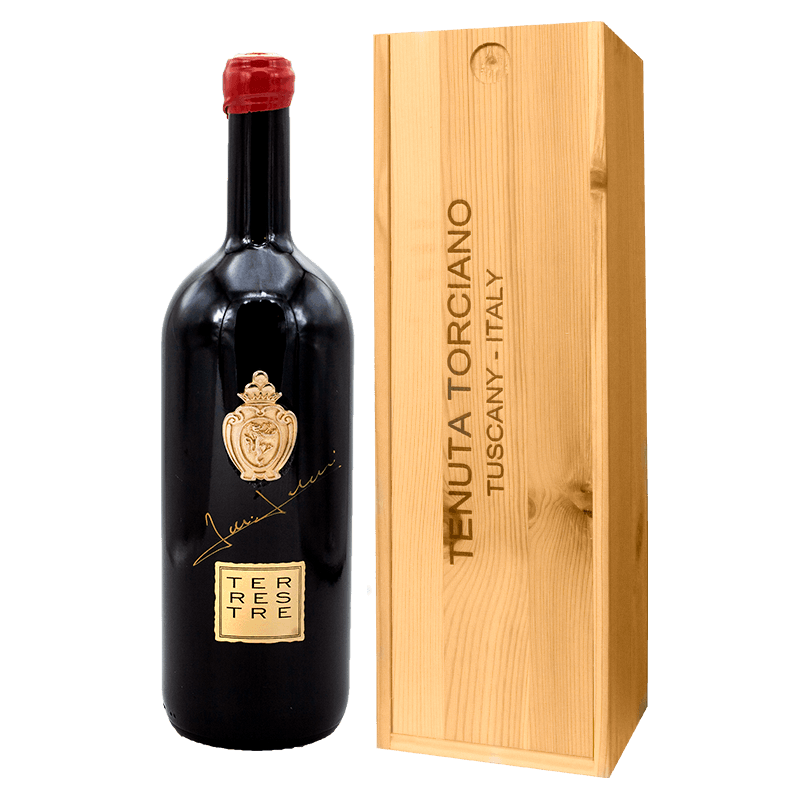
\includegraphics[width=8cm]{redwine_tuscany.png}
    \caption{An image of Tuscany red wine }
    \label{fig:1}
\end{figure}

\newpage
\section{Discussion}
Even though \cite{Zhao2015} suggest that "chitooligosaccharide should be an excellent preservative to inhibit beer-spoilage bacteria in the brewing process and in the end product" , we are not quite convinced that it will not interfere with the Reinheitsgebot. On the other hand we discovered that Charles \cite{Beer2003} does not seem to have any connection to this subject even though his name suggests so .

\par
\begin{align}
0,025*G + 0,024*H + 0,001*Y + 0,95*W = \beta eer
\end{align}






\printbibliography
\end{document}